
\section{Introduction}
\label{sec:intro}

Recently, adversarial attacks have revealed the vulnerabilities of deep learning-based models \citep{FGSM, PGD, CW_attack}, raising critical concerns in safety-important applications \citep{safe1,safe2,wang2023does}.
Thus, much research has been done on defense technologies to make deep learning more reliable\citep{2017_jpeg_defense, xie2019feature, cohen2019certified, carmon2019unlabeled, zhang2022adversarial, jin2023randomized}.
Among adversarial defense mechanisms, adversarial training is one of the most effective methods to enhance adversarial robustness \citep{pang2020bag, bai2021recent, wei2023cfa}.
However, there is a significant performance gap between large and small models in adversarial training.
Since light models with less computational complexity are preferred in practical applications, increasing the robustness of light models is necessary.
To address this, adversarial training incorporates distillation methodologies which are commonly employed to boost the performance of light or small models \citep{ard,rslad,iad,adaad}.

In the teacher-student architecture of knowledge distillation, prevailing methods leverage the teacher's features or logits \citep{hinton2015distilling, ji2021show, kim2021feature, yang2022focal}. Adversarial distillation (AD) approaches extend this paradigm by incorporating the teacher's logits as a guide within their adversarial training framework \citep{ard, iad, rslad, akd, adaad}. Recent studies have specifically focused on tailoring the inner maximization problem of adversarial training, particularly by involving the teacher model in the generation of adversarial examples \citep{rslad, adaad}.
In this paper, we exploit another knowledge of teachers: input gradient, which is highly effective in imitating the teacher.

\begin{figure}[t]
\centering
    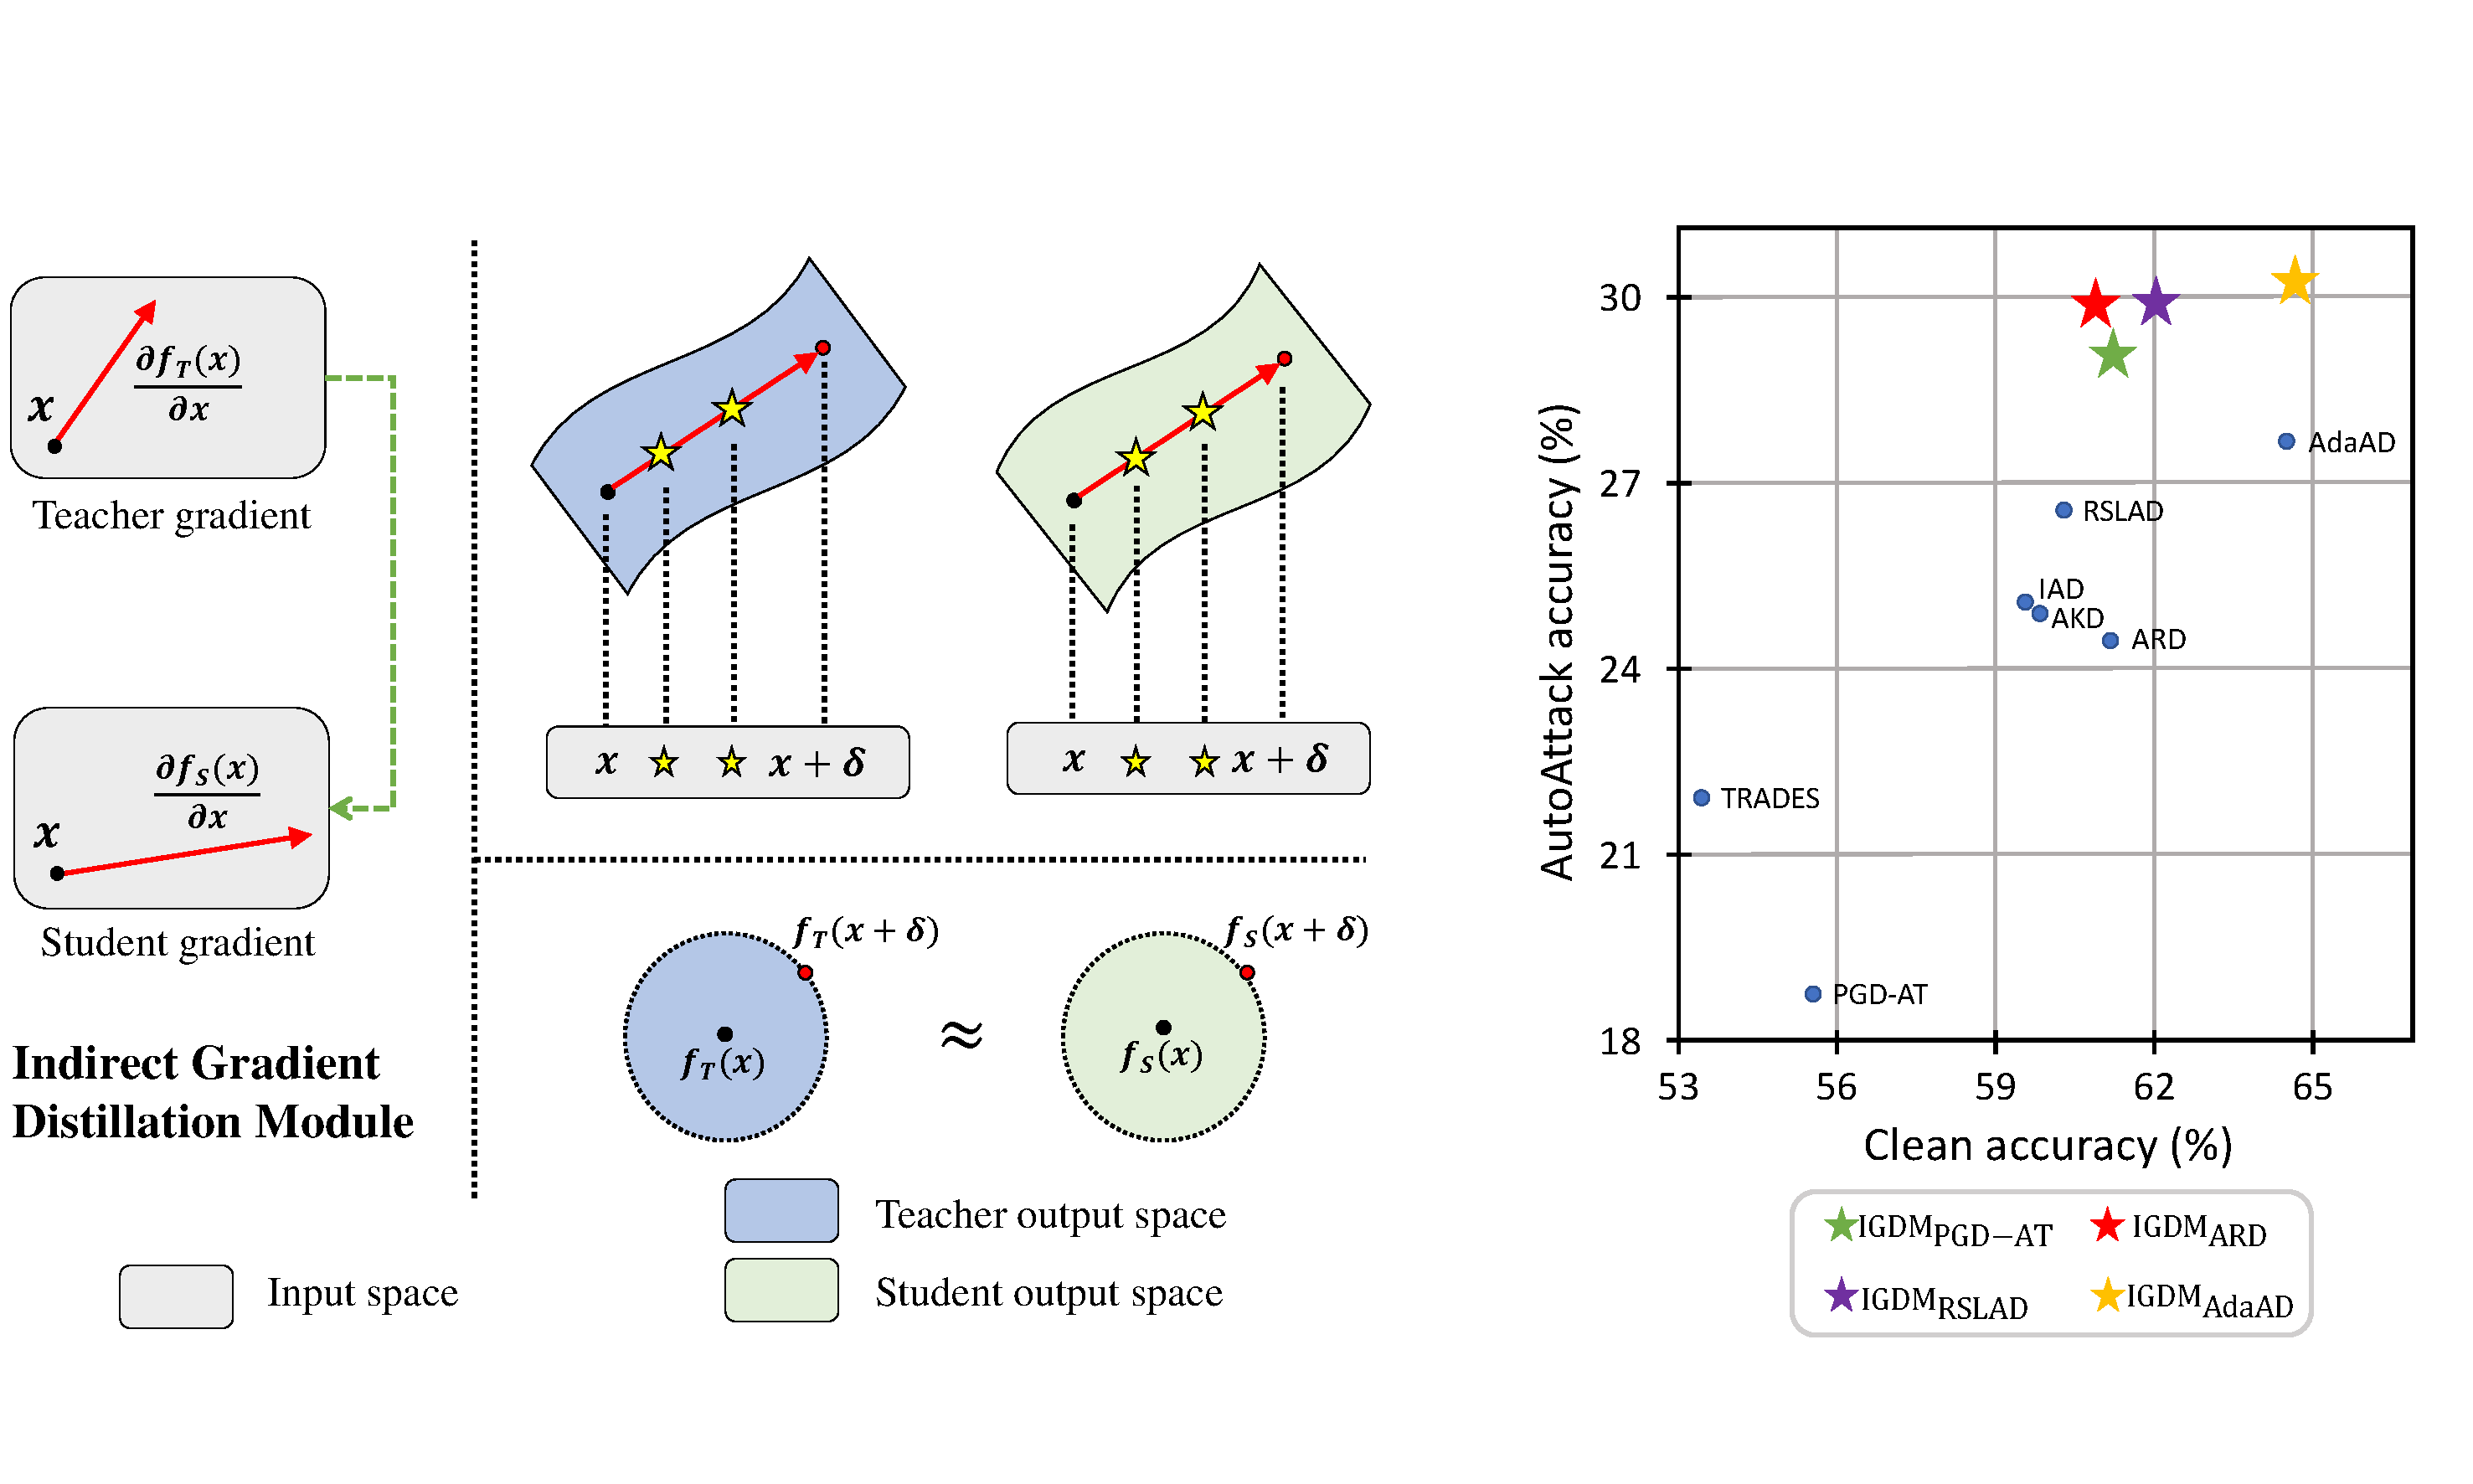
\includegraphics[width=0.95\textwidth] {figure/intro_IGDM.png}%
    \\
    \begin{minipage}[t]{.65\textwidth}
      \subcaption{Conceptual diagram of IGDM}   
       \label{fig:intro_diagram}
    \end{minipage}%
    \begin{minipage}[t]{.35\textwidth}
        \subcaption{Performance of IGDM}
       \label{fig:intro_robustness}%
    \end{minipage}
    \caption{ \textbf{(a)} We match the gradient in the input space with knowledge distillation. 
    Since adversarial robust models are locally linear, matching the gradient has the effect of matching the output points of the surrounding input marked with `stars', as illustrated in the top right figure.
    Consequently, gradient matching involves matching the teacher and student point by point in the output space, as depicted in the bottom right.
    \textbf{(b)} Clean and Autoattack accuracy on ResNet-18 with BDM-AT teacher on CIFAR-100 dataset. IGDM demonstrates significantly improved AutoAttack accuracy compared with other adversarial distillation methods.}
    \label{fig:intro}
\end{figure}


We demonstrate that matching input gradients between teacher and student contributes to point-wise alignment, allowing the student to better follow the robust teacher.
In the top right of \cref{fig:intro_diagram}, if the input gradients between the teacher and the student match as depicted in the red line, then the output of the points located on the red line, denoted as \textit{stars}, will also match.
We show that the output of random points around $x$ also becomes similar to the teacher as illustrated in the bottom right of \cref{fig:intro_diagram}.
This alignment causes the student to mimic the teacher and reduces the capacity gap between teacher and student.

In this paper, we propose \textit{Indirect Gradient Distillation Module} (IGDM), which indirectly aligns the student's gradient with that of the teacher.
We can easily match input gradients through Taylor expansion, leveraging the locally-linear properties of adversarial training.
Since existing AD methods are mainly designed to match logits, IGDM can be used in conjunction with them.
Through extensive experimental results, we verify that our method successfully complements the robustness of existing AD methods.
We significantly improve existing AD methods as depicted in \cref{fig:intro_robustness}.


Our contributions are as follows:
\begin{itemize}
\item We propose a methodology to transfer the gradient information from the teacher to the student through the exploitation of the local linearity inherent in adversarial training.
This stands in contrast to prevailing AD methods, which primarily concentrate on the distillation of logits.
\item Based on the analysis, we propose the Indirect Gradient Distillation Module (IGDM), which indirectly distills the gradient information. Its modular design allows easy integration into existing AD methods.
\item We empirically demonstrate that IGDM significantly improves robustness against various attack scenarios, datasets, student models, and teacher models.

\end{itemize}



%------------------------------------------------------------------------
